
%%%%%%%%%%%%%%%%%%%%%%%%%%%%%%%%%%%%%%%%%%%%%%%%%%

%%%%%%%%%%%%%%%%% APPENDICES %%%%%%%%%%%%%%%%%%%%%

\appendix

\section{Tidal torque \& Equations of motion}
\label{app:eom}

In this appendix, we derive the equations of motion used to simulate the asteroid angular velocity during the encounter. In particular, we describe our coordinates (section \ref{sec:coordinates}) for an encountering asteroid's position and orientation, and we parametrize its density distribution via its density moments (section \ref{sec:moments}). Then we derive an arbitrary-order equation for tidal torque (section \ref{sec:tidal-torque}) and write the equations of motion for the system (section \ref{sec:eom}).

\subsection{Coordinates}
\label{sec:coordinates}

We make use of two frames of reference to model this system. One is the ``inertial frame,'' with axes denoted by $\unit{X}$, $\unit{Y}$, $\unit{Z}$ and origin placed at the central body's centre of mass. $\unit{X}$ points from the central body to the asteroid periapse, and $\unit{Z}$ points parallel to the orbit angular momentum. We assume that the mass distribution of the central body is known in this inertial frame.

Our second frame is the ``body-fixed'' frame, denoted by $\unit{x}, \unit{y}, \unit{z}$. Each axis in this frame is aligned with a principal axis and rotates with the asteroid, with its origin at the asteroid's centre of mass. For definiteness, we define $\unit{z}$ to be the principal axis with maximal MOI (this is the short axis mode, to use the vocabulary of Ref.~\cite{kaasalainen2001interpretation}). In general, we use capital letters to denote vectors in the inertial frame and lowercase vectors to denote vectors in the body-fixed frame.

The difference between the origins of the body-fixed and inertial frames is the position of the asteroid. We represent the relative orientations by $z-y-z$ Euler angles $\alpha$, $\beta$, and $\gamma$, such that a matrix $M$ rotating from the body-fixed to the inertial frame ($M\bm{r} = \bm{R}$) is given by
\begin{equation}
M = R_z(\alpha) R_y(\beta) R_z(\gamma).
\label{eqn:euler-angles}
\end{equation}
Here, $R_i(\theta)$ is a rotation around the unit vector $i$ by $\theta$ (figure \ref{fig:euler-angles}).

\begin{figure}
    \centering
    \begin{tikzpicture}
    \draw[-{Latex[length=3mm]}] (0, 0) -- (-4, 0) node[anchor=east] {$\unit x$};
    \draw[-{Latex[length=3mm]}] (0, 0) -- (2, -3) node[anchor=west] {$\unit y$};
    \draw[-{Latex[length=3mm]}] (0, 0) -- (0, 4) node[anchor=south] {$\unit z$};
    \draw[dashed, -{Latex[length=3mm]}] (0, 0) -- (3.7, -2) node[anchor=north] {};
    \draw[line width=0.5mm,-{Latex[length=3mm]}] (0, 0) -- (-0.5, -3) node[anchor=north] {$\unit X$};
    \draw[line width=0.5mm,-{Latex[length=3mm]}] (0, 0) -- (4, 1) node[anchor=south] {$\unit Y$};
    \draw[line width=0.5mm,-{Latex[length=3mm]}] (0, 0) -- (-1.6, 2.7) node[anchor=south] {$\unit Z$};
    \draw[->] (0.5, -0.75) arc (290:302:2.5);
    \draw (0.9, -0.9) node[anchor=center] {$\alpha$};
    \draw[->] (0, 1.2) arc (130:161:1.3);
    \draw (-0.3, 1.3) node[anchor=center] {$\beta$};
    \draw[->] (0.97, -0.52) arc (330:368:1.3);
    \draw (1.4, -0.25) node[anchor=center] {$\gamma$};
    %\draw[-{Latex[length=3mm]}] (0, 0) -- (0, 4) node[anchor=south] {$\unit Z$};
    %\draw[-{Latex[length=3mm]}] (0, 0) -- (4, 0) node[anchor=west] {$\unit Y$};
    %\draw[-{Latex[length=3mm]}] (0, 0) -- (-2, -2) node[anchor=east] {$\unit X$};
    \end{tikzpicture}
    \caption{$z-y-z$ Euler angles used in this work to express the orientation of the asteroid. Orientation is expressed as a rotation from the body-fixed axes (lowercase) to the inertial axes (bold lines and uppercase). The origins are co-located for demonstration purposes.}
    \label{fig:euler-angles}
\end{figure}


\subsection{Density moments}
\label{sec:moments}

The un-normalized spherical harmonics are defined as $Y_{\ell m}(\theta, \phi) = P_{\ell m}(\cos \theta)e^{im\phi}$, where $P_{\ell m}$ are the associated Legendre Polynomials without the Condon-Shortley phase. The regular and irregular spherical harmonics are further defined as
\begin{equation}
  \begin{split}
    S_{\ell m}(\bm r) &= (-1)^m (\ell - m)! \frac{Y_{\ell m}(\unit r)}{r^{\ell+1}} \\
    R_{\ell m} (\bm r) &= (-1)^m \frac{r^\ell}{(\ell + m)!} Y_{\ell m}(\unit r).
  \end{split}
\end{equation}
These spherical harmonics obey many useful identities summarized in Ref.~\cite{Gelderen1998TheSO}, which are also useful for quantum mechanics. They were used to define the density moments in equation \ref{eqn:klm}, which can be extended to the central body:
\begin{equation}
  \begin{split}
    &J_{\ell m} = \frac{a_\mathcal{B}^{2-\ell}}{I_\mathcal{B}} \int_\mathcal{B} d^3 r \rho_\mathcal{B}(\bm r) R_{\ell m}(\bm r)\\
  \end{split}
  \label{eqn:jlm}
\end{equation}
By contrast, $J_{\ell m}$ should be computed in the inertial frame. The length scale $a_\mathcal{B}$ and MOI scale $I_\mathcal{B}$ can be defined similarly to $a_\mathcal{A}$ and $a_\mathcal{B}$ in equations \ref{eqn:aa} and \ref{eqn:ia}, but they could also be set to any other scales of the same units, e.g. $a_\mathcal{B}$ equal to the central body radius and $I_\mathcal{B} = \mu_\mathcal{B}a_\mathcal{B}^2$, where $\mu_\mathcal{B}$ is the central body mass.

Note that both $J_{\ell m}$ and $K_{\ell m}$ are unitless. We call them ``moments'' because the $R_{\ell m}(\bm r)$ contains an $r^\ell$ dependence so that $K_{\ell m}$ is the $\ell$th density moment of the asteroid.

These moments share several key properties which we discuss before continuing. Firstly, for real mass density, properties of the spherical harmonics imply that $K_{\ell m} = (-1)^m K_{\ell, -m}^*$. Therefore, the set of $K_{\ell m}$ for $\ell < \ell_\text{max}$ contains $\ell_\text{max}^2$ degrees of freedom. However, some of these degrees of freedom are redundant with the choice of coordinates: $K_{1m} = 0$ since the body-fixed frame is centred on the asteroid centre of mass. Further calculation reveals that the alignment of the body-fixed frame with the asteroid principal axes also forces $K_{21}= 0$ and $\Im K_{22}=0$. The only physical density moments for $\ell \leq 2$ are therefore $K_{22}$, $K_{20}$, and $K_{00}$. The first two are related to the MOI around each principal axis by equation \ref{eqn:moi}, while $K_{00} = \mu_\mathcal{A} a_\mathcal{A}^2 / I_\mathcal{A}$ will not be relevant to this study as it does not appear in equation \ref{eqn:tidal-torque}. 

The physical meaning of $K_{22}$ and $K_{20}$ can also be interpreted via a special case: if the asteroid is a uniform-density triaxial ellipsoid, the moments of inertia are simple to compute in terms of the semi-axis lengths and can be compared to those found in equation \ref{eqn:moi}. This yields semi-axis lengths of 
\begin{equation}
  \begin{split}
  a &= \sqrt{\frac{5}{3}}a_\mathcal{A}\sqrt{1-2K_{20}+12K_{22}}\\
  b &= \sqrt{\frac{5}{3}}a_\mathcal{A}\sqrt{1-2K_{20}-12K_{22}}\\
  c &= \sqrt{\frac{5}{3}}a_\mathcal{A}\sqrt{1+4K_{20}}.
  \label{eqn:ellipsoid-axes}
  \end{split}
\end{equation}
The higher-order moments $K_{3m}$ can be thought of loosely as measuring the large-scale asymmetries of the asteroid. An asteroid that is mirror-symmetric along the $\unit{x}$ axis (meaning $\rho_\mathcal{A}(x,y,z)=\rho_\mathcal{A}(-x,y,z)$) necessarily sets certain density moments to zero. Which density moments are zeroed by which mirror symmetries is outlined in table \ref{tab:klm-symmetries}. All $K_{3m}$ are zeroed by at least one mirror symmetry. 

\begin{table}
  \centering
  \begin{tabular}{c|ccccccc}
    \hline
    $\ell$ & $\Re K_{\ell 3}$ & $\Im K_{\ell 3}$ & $\Re K_{\ell 2}$ & $\Im K_{\ell 2}$ & $\Re K_{\ell 1}$ & $\Im K_{\ell 1}$ & $K_{\ell 0}$ \\ \hline
    0 &  &  &  &  &  &  & -\\ 
    1 &  &  &  &  & x & y & z\\ 
    2 &  &  & - & x,y & y,z & x,z & -\\ 
    3 & x,z & y,z & z & x,y,z & x & y & z\\ \hline
  \end{tabular}
  \caption{Axes of mirror symmetry that imply zeroed density moments. For example, for mirror symmetries along $\unit y$ or $\unit z$, $\Im K_{32}=0$. Mirror symmetry along $\unit x$ means $\rho_\mathcal{A}(x, y, z) = \rho_\mathcal{A}(-x, y, z)$. Dashes indicate that none of the mirror symmetries zero the moment in question. Since $r^2>0$ for $r\neq 0$, no symmetries set $a_\mathcal{A}=0$ either.}
  \label{tab:klm-symmetries}
\end{table} 

Finally, the requirement that $\rho_\mathcal{A}(\bm r) \geq 0$ everywhere restricts $K_{\ell m}$. In the case of $K_{2m}$, this fact and the constraint that $I_z$ is larger than $I_x$ or $I_y$ requires $K_{20}$ and $K_{22}$ to fall in the triangle
\begin{equation}
  -\frac{1}{4} \leq K_{20} \leq 0, \qquad |K_{22}| \leq -\frac{K_{20}}{2}.
  \label{eqn:parameter-bounds}
\end{equation}
An analytical constraint on $K_{3m}$ based on this property is more difficult to derive, but in practice, we also observe that $|K_{3m}| < 0.01$.




\subsection{Tidal torque}
\label{sec:tidal-torque}

Derivations for the tidal torque experienced by a rigid body in the gravitational field of a larger mass have been computed by several previous studies \cite{paul88,HouMar2017,BOUE2009750, ashenberg07}, often in terms of the MOI of the rigid body (or higher order moments of inertia), and to varying degrees of precision. A simple, first-order derivation is also easily computable in terms of the asteroid MOI in the inertial frame.

Here, we present a new derivation of the tidal torque to arbitrary orders in terms of the density moments of an asteroid defined in section \ref{sec:moments}. These density moments can be pre-computed and do not have to be re-evaluated every time-step.

The gravitational potential energy of the central body is, in its most general form,
\begin{equation}
V(\bm R') = -G\int_\mathcal{B} d^3 R \rho_\mathcal{B}(\bm R) \frac{1}{|\bm{R}-\bm{R'}|}.
\label{eqn:first-pe}
\end{equation}
where $\rho_\mathcal{B}$ is the density distribution of the central body and $\mathcal{B}$ indicates the central body's volume. All vectors here are written in the inertial frame. Given $|\bm{R}| < |\bm{R'}|$, Ref.~\cite{Gelderen1998TheSO} gives the identity
\begin{equation}
  \frac{1}{|\bm R - \bm R'|} = \sum_{\ell, m} R_{\ell m}(\bm R) S_{\ell m}^*(\bm R'),
  \label{eqn:ylm-expansion}
\end{equation}
where the sum is shorthand for $\sum_{\ell, m} = \sum_{\ell = 0}^\infty \sum_{m=-\ell}^\ell$.

Incidentally, it is the $|\bm R| < |\bm R'|$ assumption that inspires the assumption that there are ``no \textit{distant} perturbing objects'' (section \ref{sec:methods}). If a perturbing object such as a moon is not distant (i.e., it is closer to the system center of mass than the asteroid perigee so that $|\bm R| < |\bm R'|$ always), then it can be absorbed into $J_{\ell m}$ by equation \ref{eqn:jlm} and the assumptions of this derivation are not violated.

We are interested in translating the potential energy of equation \ref{eqn:first-pe} to the body-fixed frame. To do this, we let $\bm{R'} = \bm D + \bm U$, where $\bm D$ is the location of the asteroid in the inertial frame. We further define $\bm U = M\bm u$, where $\bm u$ is in the body-fixed frame and $M$ is the rotation matrix given by the Euler angles $\alpha$, $\beta$, and $\gamma$ (see section \ref{sec:coordinates}). The translation from $\bm {R'}$ to $\bm U$ is then attained by the identity 
\begin{equation}
  S_{\ell m}(\bm R') = \sum_{\ell', m'} (-1)^{\ell'}R^*_{\ell' m'}(\bm U)S_{\ell+\ell', m + m'} (\bm D),
  \label{eqn:ylm-translation}
\end{equation}  
provided by Ref.~\cite{Gelderen1998TheSO}, and from $\bm U$ to $\bm u$ is given by
\begin{equation}
  \begin{split}
    Y_{\ell m}(M\bm u) = \sum_{m'=-\ell}^\ell & (-1)^{m+m'}\sqrt{\frac{(\ell-m')!(\ell+m)!}{(\ell+m')!(\ell-m)!}} \\
    & \times \mathcal{D}^\ell_{mm'}(M)^* Y_{\ell m'}(\bm u).\\
  \end{split}
  \label{eqn:ylm-rotation}
\end{equation}
Here, $\mathcal{D}^\ell_{mm'}(M)$ are the Wigner-$D$ matrices, which are determined by the Euler angles $\alpha$, $\beta$, and $\gamma$ of $M$.

Equations \ref{eqn:first-pe} to \ref{eqn:ylm-rotation} then provide formula for $V(\bm u)$ expressed as a sum of integrals over $\mathcal{B}$ of the central body density $\rho_\mathcal{B}(\bm R)$ times $R_{\ell m}(\bm R)$. These are expressed via equation \ref{eqn:jlm} as $J_{\ell m}$.

The tidal torque experienced by the asteroid (in the body-fixed frame) is given by
\begin{equation}
  \bm{\tau}(\bm u) = \int_\mathcal{A} d^3 u \rho_\mathcal{A}(\bm u) (\bm u \times (-\nabla_{\bm u} V(\bm u)))
\end{equation}
where $\rho_\mathcal{A}$ is the density distribution of the asteroid and $\mathcal{A}$ indicates the volume of the asteroid. Making use of one more identity concerning the derivatives of spherical harmonics:
\begin{equation}
  \begin{split}
  \bm u \times \nabla R_{\ell m}(\bm u)=&\frac{1}{2}\Big[(i\unit x - \unit y)(\ell-m+1)R_{\ell,m-1}(\bm u)\\
  &+(i\unit x+\unit y)(\ell+m+1)R_{\ell,m+1}(\bm u)\\
  & +2im\unit z R_{\ell m}(\bm u)\Big],
  \end{split}
\end{equation}
tidal torque can now be expressed as a function only of the constants $J_{\ell m}$, $K_{\ell m}$, $a_\mathcal{A/B}$, $I_\mathcal{A/B}$, and the asteroid orientation and position (equation \ref{eqn:tidal-torque}). Some $K_{\ell m}$ terms are written in this equation with $|m|>\ell$; these should all be taken to be zero.

\subsection{Equations of motion}
\label{sec:eom}


The equations of motion of the asteroid position $\bm D$ are given by Newton's law of gravitation
\begin{equation}
  \dot{\bm V} = -\frac{G \mu_\mathcal{B}}{D^3} \bm D \qquad \dot{\bm D} = \bm V
  \label{eqn:pos-eom}
\end{equation}
where $\bm V$ is the asteroid velocity in the inertial frame. Rather than derive equations of motion for the Euler angles (which suffer from gimbal lock), we instead represent the orientation of the asteroid with a quaternion $\quat q$ which can be converted into Euler angles to compute $\mathcal{D}(\alpha, \beta, \gamma)$. This quaternion evolves as 
\begin{equation}
  \dot{\quat q} = \frac{1}{2}\quat q\quat \omega.
  \label{eqn:quat-eom}
\end{equation}
for angular velocity $\bm \omega$ given in the body-fixed frame. The equations of motion of $\bm \omega$ in turn are given by
\begin{equation}
  \begin{split}
    I_x \dot \omega_x - \omega_y \omega_z (I_y - I_z) &= \tau_x\\
    I_y \dot \omega_y - \omega_z \omega_x (I_z - I_x) &= \tau_y\\
    I_z \dot \omega_z - \omega_x \omega_y (I_x - I_y) &= \tau_z.
  \end{split}
  \label{eqn:omega-eom}
\end{equation}
Equations \ref{eqn:tidal-torque}, \ref{eqn:moi}, and \ref{eqn:pos-eom} to \ref{eqn:omega-eom} form a set of non-linear, first-order coupled differential equations in which can be numerically integrated. They are expressed in terms of the physical parameters $I_\mathcal{A/B}$, $a_\mathcal{A/B}$, $J_{\ell m}$, and $K_{\ell m}$ which are constant if the asteroid is rigid and the central body does not rotate.





\section{Additional density distribution models}
\label{app:more-models}

Two models were discussed in section \ref{sec:density-distro} to translate density moment constraints into density distribution constraints. Here we outline two additional models, the nearly-uniform and the harmonic models, which are less conventional but still useable for extracting density distribution properties. Unlike the finite element and lumpy models discussed in the main text, these models will yield smooth distributions with no discrete transitions. They also rely on a known surface for the asteroid.

\subsection{Nearly-uniform model}
In this ``nearly-uniform'' model, we seek to pick one density distribution from the many distributions consistent with the data by maximizing a prior distribution $f[\rho(\bm r)]$, which can be chosen manually. Any prior distribution can be chosen, but the following prior is both interesting and numerically efficient.

As part of our prior, we require that the asteroid density distribution satisfy $I_\mathcal{A} = \mu_\mathcal{A} a_\mathcal{A}^2$. This constraint is desirable as it is obeyed for uniform density distributions. To define the prior, we divide the asteroid into $n \gg 1$ small regions of volume $V$, each with position $\bm r_i$ and density $\rho_i = \delta_i + 1$. Setting the mass of the asteroid equal to its volume, the average density is 1, so $\delta_i$ is the difference between the average and local density. We set $f[\rho(\bm r)]$ to be a multivariate-Gaussian distribution on $\delta_i$, centred on zero to minimize non-uniformity, i.e.
\begin{equation}
  f[\rho(\bm r)] \propto \prod_i \exp\parens{-\frac{\delta_i^2}{2\sigma^2}} \implies \ln f[\rho(\bm r)] \simeq -\sum_i \delta_i^2
  \label{eqn:nu-f}
\end{equation}
where $\sigma$ is an irrelevant constant. The density moments, MOI scale, and mass are 
\begin{equation}
  K_{\ell m} = \frac{V}{\mu_\mathcal{A}a_\mathcal{A}^{\ell}} \sum_i (\delta_i + 1) R_{\ell m}(\bm r_i)
  \label{eqn:nu-klm}
\end{equation}
\begin{equation}
  I_\mathcal{A} = \mu_\mathcal{A} a_\mathcal{A}^2 = V \sum_i (\delta_i + 1) r_i^2
  \label{eqn:nu-ia}
\end{equation}
\begin{equation}
  \mu_\mathcal{A} = V\sum_i (\delta_i + 1) \implies 0 = \sum_i \delta_i.
  \label{eqn:nu-mass}
\end{equation}
Writing $\delta_i$ as an $n$-dimensional vector $\bm \delta$, equation \ref{eqn:nu-klm} is a matrix equation for $K_{\ell m}$, and equations \ref{eqn:nu-ia} and \ref{eqn:nu-mass} are vector dot product equations. Combining $K_{\ell m}$, $I_\mathcal{A}$, and $0$ into a single vector $\bm K$, these equations can be written as a single underdetermined matrix equation we denote as 
\begin{equation}
  \bm K = M \bm \delta + \bm C,
  \label{eqn:nu-matrix}
\end{equation}
where the components of constant matrix $M$ and constant vector $\bm C$ are known given a fixed layout of the $n$ regions. Some of the components of $\bm K$, such as $I_\mathcal{A}$, $\mu_\mathcal{A}$, and $K_{1m}$, are constraints. We treat the other components as parameters of the model. The task is then to find $\bm \delta$ that satisfies equation \ref{eqn:nu-matrix} and maximizes $f(\bm \delta)$. But the form of equation \ref{eqn:nu-f} shows that the maximum of $\ln f$ (also the maximum of $f$) is the minimum of $|\bm \delta|^2$. This shortest value of $\bm \delta$ that obeys equation \ref{eqn:nu-matrix} is given by the Moore-Penrose inverse:
\begin{equation}
  \bm \delta = M^+ (\bm K - \bm C); \qquad M^+ = M^\dagger(M M^\dagger)^{-1}
  \label{eqn:nu-delta}
\end{equation}
where $M^\dagger$ is the adjoint of $M$.

The prior distribution on $\rho(\bm r)$ discussed in section \ref{sec:fit} can be implemented by individually checking the components $\bm \delta$ computed by equation \ref{eqn:nu-delta} and confirming that $1 + \delta_i$ lies within the acceptable range of densities.
 can be implemented by individually checking the components $\bm \delta$ computed by equation \ref{eqn:nu-delta} and confirming that $1 + \delta_i$ lies within the acceptable range of densities.


\subsection{Harmonic model}
This the ``harmonic model'', we limit ourselves to density distributions that are harmonic; i.e., they satisfy $\nabla^2 \rho(\bm r) = 0$. We have no physical justification for why this assumption should be true, but it is useful as a simplification to gain qualitative insight into the properties of the asteroid density distribution.

A harmonic density distribution can be expanded in terms of the spherical harmonics as $\rho(\bm r) = \sum_{\ell m} C_{\ell m} R_{\ell m}(\bm r)^*$ where $C_{\ell m}$ are complex, free parameters. This series can be truncated at some maximum $\ell$. The density moments, MOI scale, and mass can then be explicitly computed as a function of $C_{\ell m}$:
\begin{equation}
  K_{\ell m} = \frac{a_\mathcal{A}^{2-\ell}}{I_\mathcal{A}} \sum_{\ell m} C_{\ell' m'} \int_\mathcal{A} d^3 r R_{\ell' m'}(\bm r)^* R_{\ell m}(\bm r)
  \label{eqn:harmonic-klm}
\end{equation}
\begin{equation}
  I_\mathcal{A} = \sum_{\ell m} C_{\ell m} \int_\mathcal{A} d^3 r R_{\ell m}(\bm r)^* r^2
  \label{eqn:harmonic-ia}
\end{equation}
\begin{equation}
  \mu_\mathcal{A} = \sum_{\ell m} C_{\ell m} \int_\mathcal{A} d^3 r R_{\ell m}(\bm r)^*.
  \label{eqn:harmonic-mass}
\end{equation}
These integrals can be pre-computed given a known asteroid shape $\mathcal{A}$, so that computing $C_{\ell m}$ to match a given $K_{\ell m}$ is fast. Furthermore, their values when $\mathcal{A}$ is spherical gives us insight into the influence of $K_{\ell m}$ on density distributions. In this case, $I_\mathcal{A} \propto C_{00}$ and the integral of equation \ref{eqn:harmonic-klm} is non-zero only when $\ell' = \ell$ and $m'=m$. Therefore, $C_{\ell m}$ is proportional to $K_{\ell m}$. The density distribution can be immediately visualized given the density moments as a sum of the solid spherical harmonics weighted by $K_{\ell m}$. When the asteroid is non-spherical, the shape itself contributes to $K_{\ell m}$ so as to break this picture.

Imposing constraints on these moments is also necessary. The choice of mass is enforced via equation \ref{eqn:harmonic-mass}. We impose bounds on $\rho(\bm r)$ by acknowledging that harmonic functions such as $\rho(\bm r)$ in a region such as $\mathcal{A}$ attain their maxima on the boundary of the region, so that it is only necessary to ensure that $\rho$ lies within the allowed range on the asteroid boundary rather than within the entire asteroid. This can be done by parametrizing the asteroid surface as a function of two variables (e.g., latitude and longitude) and minimizing and maximizing $\rho$ with respect to those variables, ensuring these minima and maxima are within the allowed range.




\section{Comparing orientation and angular velocity data}

To extract the density distribution of an asteroid, the main text assumes that the angular velocity data of the asteroid is observable. It is possible that the orientation of the asteroid may be better constrained by observations than angular velocity. In this appendix, we generate an orientation data set for the reference asteroid flyby, extract a density distribution from it, and compare the results to distributions extracted from angular velocity data.

\subsection{Uncertainty model}
The likelihood used by the MCMC (equation \ref{eqn:log-likelihood}) requires redefinition in order to extract density moments from orientation data. This requires a new model for the uncertainty of orientation observations.

For the sake of this appendix, we will assume that all observations of orientation $O$ differ from the true orientation $O^*$ by a rotation by some angle $\phi$ around an axis drawn from a uniform distribution on the unit sphere, where $\phi$ is drawn from a normal distribution with mean zero and standard deviation $\sigma_\phi$. Expressing orientation as a quaternion $\quat q = q_r + q_i \bm i + q_j \bm j + q_k \bm k$, $\phi$ can be extracted and the likelihood written as 
\begin{equation}
  \ln \mathcal{L} = -\frac{2}{\sigma_\phi^2}\sum_{i=0}\parens{\cos^{-1}\left|\brackets{\quat q_i (\quat q_i^*)^{-1}}_r\right|}^2
  \label{eqn:orientation-like}
\end{equation}
where $\quat q_i$ is the $i$th quaternion in the data set measured in the inertial frame, and $\quat q_i^*$ is the true quaternion. It is assumed that both quaternions have norm one.

\subsection{Moment uncertainty comparison}
With the likelihood defined, we generate both angular velocity and orientation data for the asymmetric reference asteroid configuration and extract $K_{\ell m}$ means and uncertainties for both data sets via the fit method defined in the main text. Due to the different uncertainty models used for the orientation and angular velocity data sets, this set-up does not allow direct comparison between the sizes of moment uncertainty for both data sets. If one data set yields more precise moments than the other, one could not determine whether the effect is due to increased observational precision in the data set or the use of a data type that better constrains density moments. However, the relative uncertainty of moments can be compared between the two data sets.

To make this comparison, we compute moment uncertainties $\sigma(K_{\ell m})$ for both data sets and also compute the mean value of $\sigma(K_{\ell m})$ over all fit parameters. We then scale the moment uncertainties attained from the angular velocity data set so that the mean uncertainty of its parameters is equal to that of the orientation data set. This is equivalent to simply choosing observational uncertainties for the angular velocity data set which yield density moments to the same precision as the observational data set, because figure \ref{fig:scan-observational} shows that density moment uncertainty $\sigma(K_{\ell m})$ is proportional to observational uncertainty. The resulting PPDs for the density moments of both data sets are displayed in figure \ref{fig:orientation-unc}, as well as their mean values relative to the true values.

\begin{figure*}
  \centering
  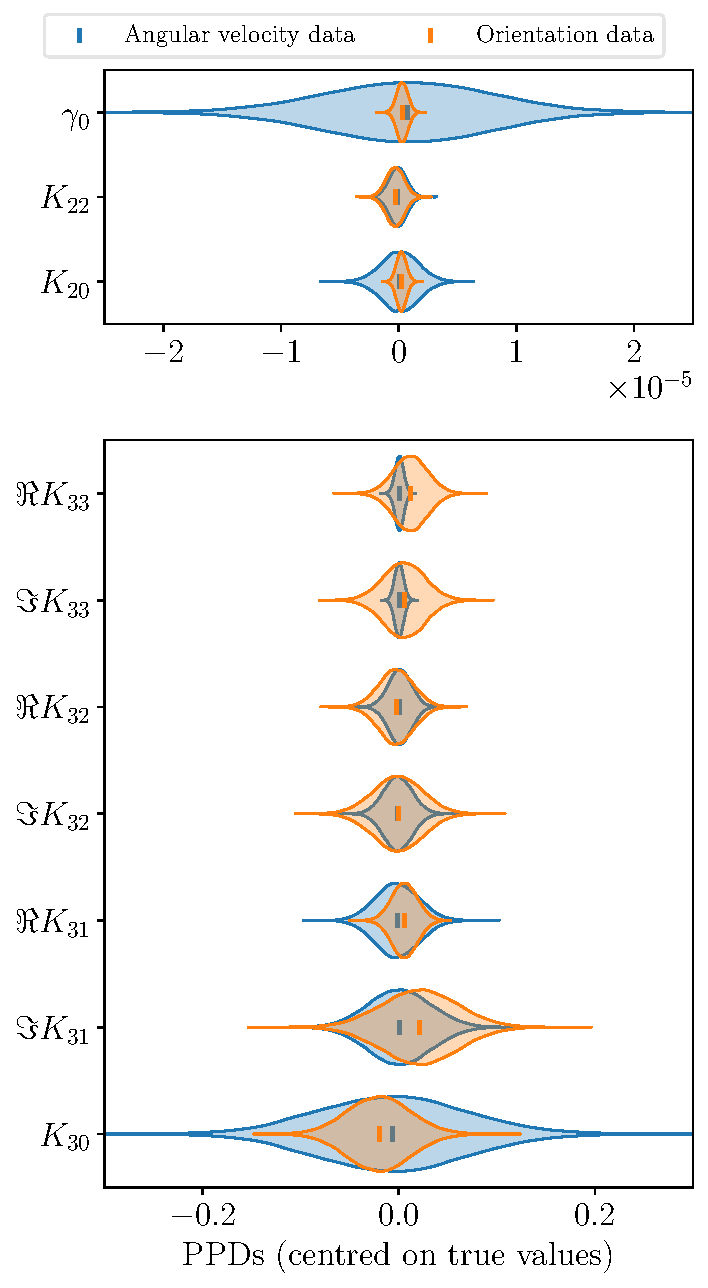
\includegraphics[width=0.75\linewidth]{figs/orientation-unc}
  \caption{PPDs for each parameter as extracted from angular velocity (blue) and orientation (orange) data. First order parameters are shown in the left panel and second-order parameters in the right. Mean values are also shown as horizontal lines. Both data produce similar constraints on parameters, except in the case of $\gamma_0$.}
  \label{fig:orientation-unc}
\end{figure*}

The figure demonstrates that using orientation data rather than angular velocity data does not greatly affect the relative uncertainties of density moments, except in the case of $\gamma_0$. This is expected due to the following argument. If the initial orientation of the asteroid is known, then the orientation of the next data point can be determined by knowledge of the asteroid's angular velocity at that moment. Thus, an orientation data set can be produced from an angular velocity data set and vice versa given an initial asteroid orientation. This initial orientation is defined up to $\gamma_0$ by the assumption of no initial tumbling, so that the orientation data set will affect $\sigma(\gamma_0)$ most strongly. A smaller effect observed in figure \ref{fig:orientation-unc} is that the orientation data set yields similar uncertainties for all density moments of fixed $\ell$, whereas the angular velocity data set tends to yield larger uncertainties for small $|m|$.

\subsection{Density uncertainty comparison}






% \section{Dependence of the cadence cut-off on time scales}
% \label{app:cadence-tests}

% In section \ref{sec:scan-cadence}, we noted that moment uncertainty as a function of observation cadence $\Delta t$ increases suddenly near $\Delta t_\text{cut-off} \approx 30-40$ min. By dimensional analysis, $\Delta t_\text{cut-off}$ depends both on the asteroid period $P_\omega$ and the orbital time scales. In this appendix, we assess the relationship between $\Delta t_\text{cut-off}$ and these time scales by measuring moment uncertainty as a function of cadence at different values of these time scales. However, changing the time scales also affects the moment uncertainty directly, obscuring the cadence dependence of the moment uncertainty. Figure \ref{fig:scan-period} indicates that $P_\omega$ only slightly affects moment uncertainty as long as $P_\omega$ is not too small, so we neglect this obscuring effect in the case of $P_\omega$. To assess the dependence of $\Delta t$ on the orbital time scales, we fix the orbit shape and simulate the asteroid as following the orbit at different speeds. This process is unphysical, but it has the advantage of keeping all encounter parameters fixed except for the time the asteroid spends in the orbit, thereby isolating the orbital time scale. We parametrize this change $v_\text{orbit} / v_\text{physical}$, which is large for an artificially fast encounter, low for an artificially slow encounter, and 1 for a physical encounter.

% In figure \ref{fig:cad-contour}, we display contour plots of moment uncertainty $\sigma(K_{\ell m})$ of the fit parameters as a function of both cadence $\Delta t$ and $P_\omega$ and the relative orbit speed $v_\text{orbit} / v_\text{physical}$. Superimposed is the weak Both panels show the same sudden increase in posterior uncertainty we named $T_\text{cad}$, located around the region where $\sigma_\rho / \rho = 100\%$ and now visible as a function of frequency and relative orbit speed. In all cases, the value of $\gamma_0$ was set so that all data points achieve the same value of $\gamma$ at perigee.

% \begin{figure*}
%   \centering
%   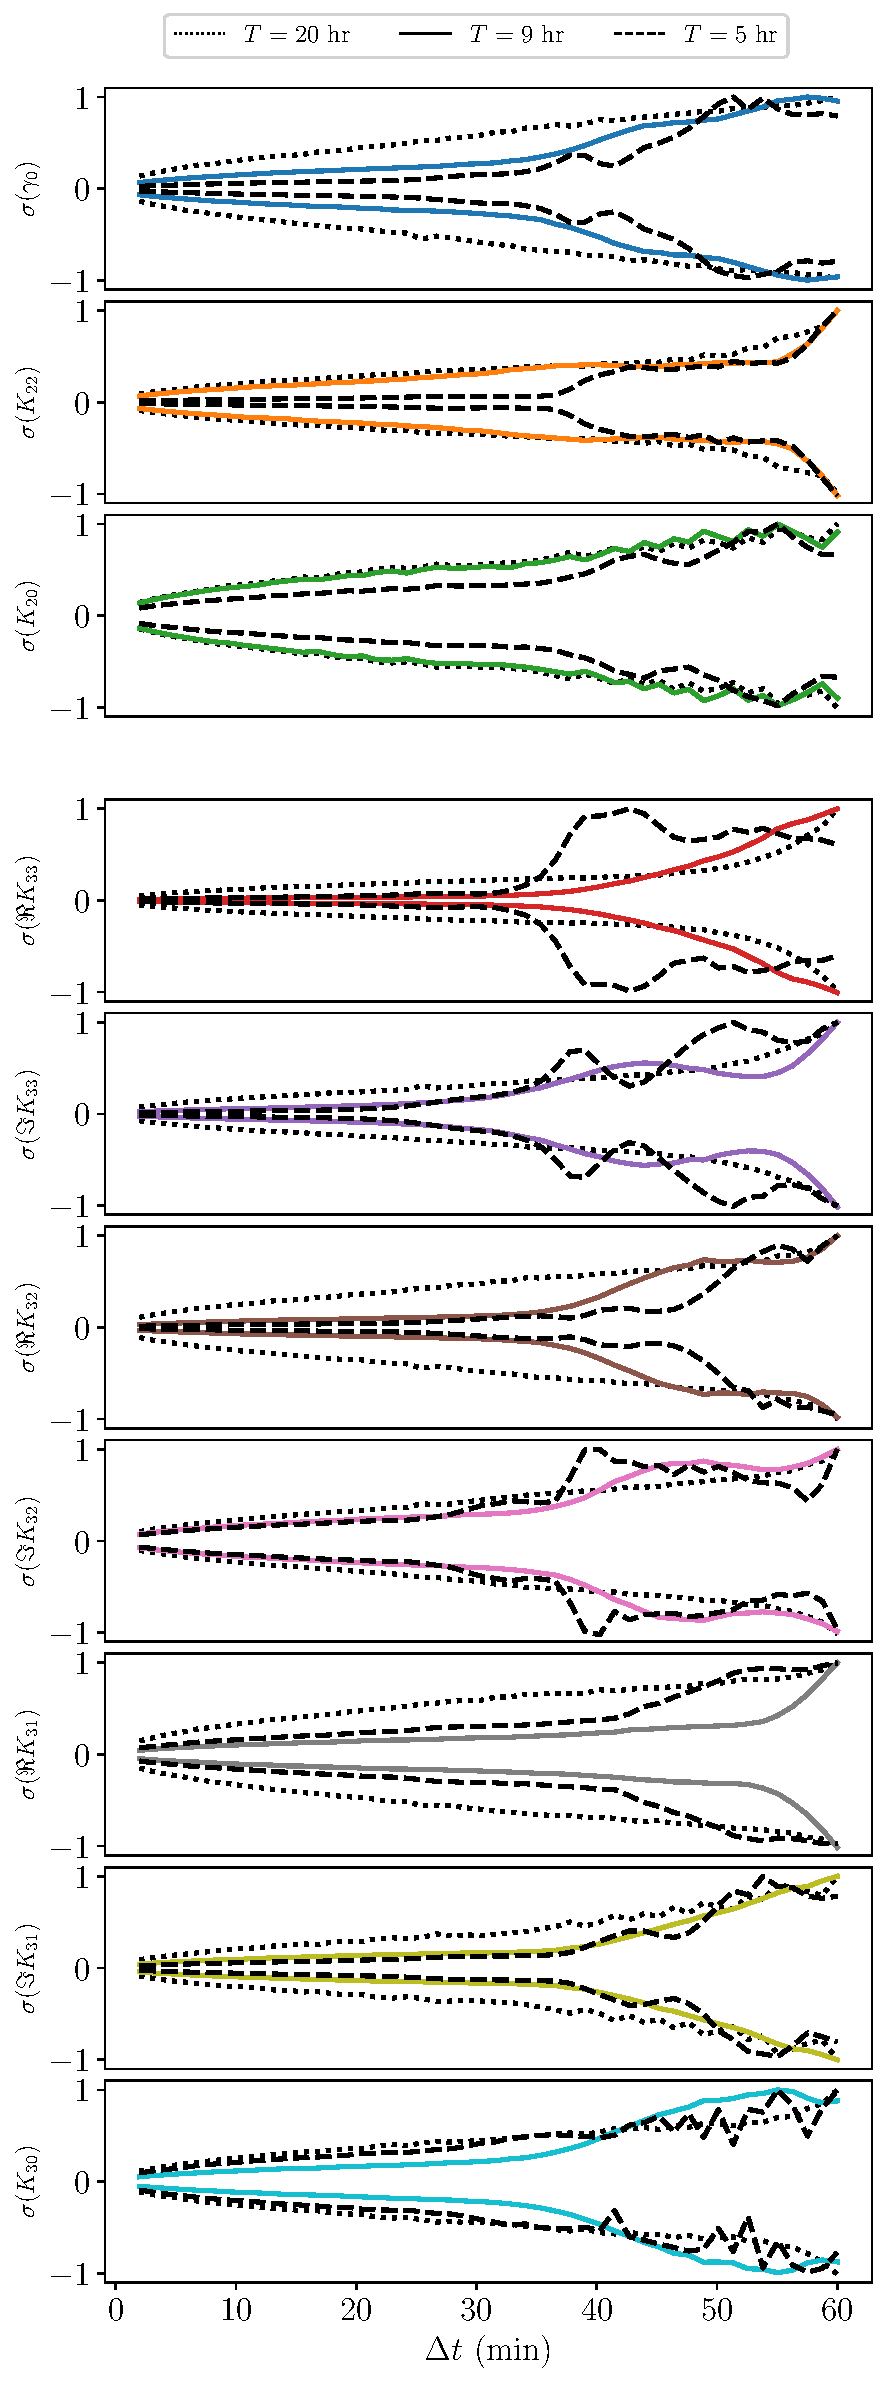
\includegraphics[width=0.48\textwidth]{figs/cad-period.pdf}\hfill
%   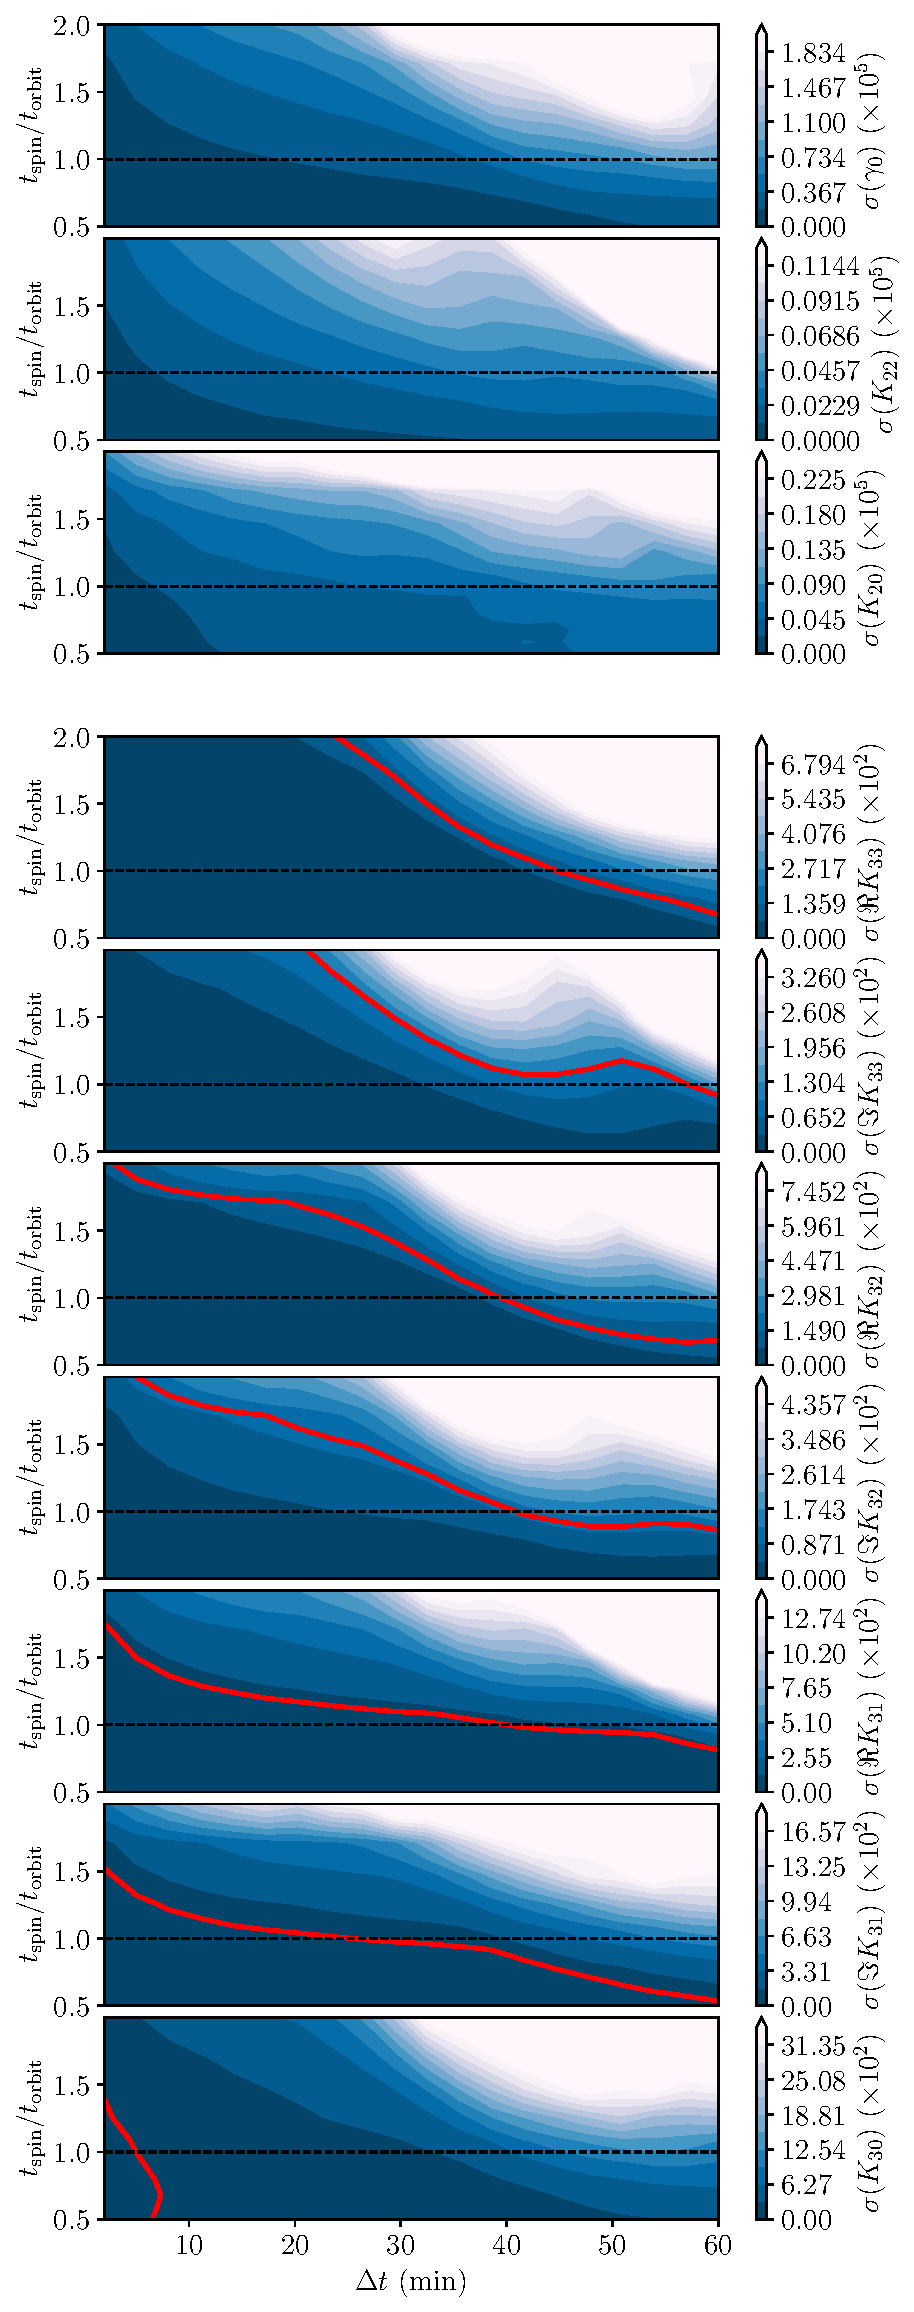
\includegraphics[width=0.48\textwidth]{figs/cad-speed.pdf}
%   \caption{Contour plots showing posterior uncertainties as a function of cadence $\Delta t$ and dynamical time scales for the encounter: rotational period $P_\omega$ (\textit{left}) and the relative speed of the orbit (\textit{right}; see text for a definition). The reference values of $P_\omega=9$ hr and $t_\text{spin}/t_\text{orbit}=1$ are shown as dotted lines. The solid (dotted) red line represents the $\sigma_\rho / \rho = 100\%$ (20\%) threshold. Cadence cut-off depends strongly on both $P_\text{omega}$ and $t_\text{spin}/t_\text{orbit}=1$.}
%   \label{fig:cad-contour}
% \end{figure*}

% Figure \ref{fig:cad-contour} demonstrates that large rotational period produces high $T_\text{cad}$. The dependence on $P_\omega$ agrees with the fact that large rotational periods for fixed cadence lead to better posterior uncertainty, discussed in section \ref{sec:scan-period}. The figure also demonstrates that for large $P_\omega$, $T_\text{cad}$ depends less strongly on $P_\text{omega}$ and may even reverse its dependence such that increasing $P_\text{omega}$ decreases $T_\text{omega}$. In all cases except $\Re K_{33}$, at least constant-$\sigma(K_{\ell m})$ contour is seen to curve back such that $\Delta t$ decreases as a function of $P_\text{omega}$ for large $P_\text{omega}$. In these regions the cadence cut-off also dulls, as shown by the spreading of the constant-$\sigma(K_{\ell m})$ contours in this region.

%  The relative orbit speed $t_\text{spin} / t_\text{orbit}$ was defined by un-physically increasing or decreasing the time at which the asteroid moved through the orbit determined by the equations of motion (but leaving the orbit shape unchanged). The equations of motion affecting the orientation and spin of the asteroid however were unaffected. $t_\text{spin} / t_\text{orbit} > 1$ corresponds to a faster orbit, and $t_\text{spin} / t_\text{orbit} < 1$ corresponds to a slower orbit. With this unphysical process, we isolate the effect of the amount of time spent near perigee on posterior uncertainty, without inheriting additional affects that would have been caused by the orbit changing shape.

% The right panel of figure \ref{fig:cad-contour} shows a stronger and more monotonic dependence of $T_\text{cad}$ on $t_\text{spin} / t_\text{orbit}$. It appears that even slightly slower orbits sharply increases $T_\text{cad}$. This effect is both due to the asteroid spending greater time in the high-torque, near-perigee region, and the larger data set that can be collected for slow orbits. However, if the orbit speed is changed by adjusting its parameters ($v_\infty$, $r_p$) or the central body mass $\mu_\mathcal{B}$, then the orbit shape will also change. This induces other effects studied in the main text and will complicate the trend observed here. Unlike the $P_\omega$ case, the cadence cut-off does not visibly broaden as a function of $t_\text{spin} / t_\text{orbit}$. It appears that the increased orbit speed merely shifts $T_\text{cad}$ rather than changing its sharpness.




\section{Animated density distributions}

This appendix contains animations to better display the density distributions shown in the main text. Each frame represents a cross section perpendicular to the $\unit z$-axis, starting with negative $z$ and ending with positive $z$. All densities are divided by the mean asteroid density.

\begin{figure*}
  \textbf{Please see the published version of the paper for these animations, or find them online at the following links.}

  \href{https://github.com/jack-dinsmore/asteroid-tidal-torque/tree/main/paper/gifs/asym-fe-d.mp4}{FE asymmetric density} \hfill
  \href{https://github.com/jack-dinsmore/asteroid-tidal-torque/tree/main/paper/gifs/asym-fe-s.mp4}{FE asymmetric deviation} \hfill
  \href{https://github.com/jack-dinsmore/asteroid-tidal-torque/tree/main/paper/gifs/asym-fe-u.mp4}{FE asymmetric uncertainty} \hfill
  \href{https://github.com/jack-dinsmore/asteroid-tidal-torque/tree/main/paper/gifs/asym-fe-r.mp4}{FE asymmetric significance}

  \href{https://github.com/jack-dinsmore/asteroid-tidal-torque/tree/main/paper/gifs/asym-l-d.mp4}{Lumpy asymmetric density} \hfill
  \href{https://github.com/jack-dinsmore/asteroid-tidal-torque/tree/main/paper/gifs/asym-l-s.mp4}{Lumpy asymmetric deviation} \hfill
  \href{https://github.com/jack-dinsmore/asteroid-tidal-torque/tree/main/paper/gifs/asym-l-u.mp4}{Lumpy asymmetric uncertainty} \hfill
  \href{https://github.com/jack-dinsmore/asteroid-tidal-torque/tree/main/paper/gifs/asym-l-r.mp4}{Lumpy asymmetric significance}

  \href{https://github.com/jack-dinsmore/asteroid-tidal-torque/tree/main/paper/gifs/sym-fe-d.mp4}{FE symmetric density} \hfill
  \href{https://github.com/jack-dinsmore/asteroid-tidal-torque/tree/main/paper/gifs/sym-fe-s.mp4}{FE symmetric deviation} \hfill
  \href{https://github.com/jack-dinsmore/asteroid-tidal-torque/tree/main/paper/gifs/sym-fe-u.mp4}{FE symmetric uncertainty} \hfill
  \href{https://github.com/jack-dinsmore/asteroid-tidal-torque/tree/main/paper/gifs/sym-fe-r.mp4}{FE symmetric significance}

  \href{https://github.com/jack-dinsmore/asteroid-tidal-torque/tree/main/paper/gifs/sym-l-d.mp4}{Lumpy symmetric density} \hfill
  \href{https://github.com/jack-dinsmore/asteroid-tidal-torque/tree/main/paper/gifs/sym-l-s.mp4}{Lumpy symmetric deviation} \hfill
  \href{https://github.com/jack-dinsmore/asteroid-tidal-torque/tree/main/paper/gifs/sym-l-u.mp4}{Lumpy symmetric uncertainty} \hfill
  \href{https://github.com/jack-dinsmore/asteroid-tidal-torque/tree/main/paper/gifs/sym-l-r.mp4}{Lumpy symmetric significance}

  \caption{Density distributions extracted via the finite element model for the asymmetric (\textit{top two rows}) and symmetric (\textit{bottom two rows}) reference asteroids. The finite element model (\textit{first and third rows}) and the lumpy model (\textit{second and fourth rows}) are employed. From left to right, the densities, deviations from the true density, uncertainties, and significance of the deviations are plotted. Animated form of figure \ref{fig:den-uniform}.}
  \label{fig:animated-uniform}
\end{figure*}

\begin{figure*}
  \textbf{Please see the published version of the paper for these animations, or find them online at the following links.}

  \href{https://github.com/jack-dinsmore/asteroid-tidal-torque/tree/main/paper/gifs/move-fe-d.mp4}{FE density} \hfill
  \href{https://github.com/jack-dinsmore/asteroid-tidal-torque/tree/main/paper/gifs/move-fe-s.mp4}{FE deviation} \hfill
  \href{https://github.com/jack-dinsmore/asteroid-tidal-torque/tree/main/paper/gifs/move-fe-u.mp4}{FE uncertainty} \hfill
  \href{https://github.com/jack-dinsmore/asteroid-tidal-torque/tree/main/paper/gifs/move-fe-r.mp4}{FE significance}

  \href{https://github.com/jack-dinsmore/asteroid-tidal-torque/tree/main/paper/gifs/move-l-d.mp4}{Lumpy density} \hfill
  \href{https://github.com/jack-dinsmore/asteroid-tidal-torque/tree/main/paper/gifs/move-l-s.mp4}{Lumpy deviation} \hfill
  \href{https://github.com/jack-dinsmore/asteroid-tidal-torque/tree/main/paper/gifs/move-l-u.mp4}{Lumpy uncertainty} \hfill
  \href{https://github.com/jack-dinsmore/asteroid-tidal-torque/tree/main/paper/gifs/move-l-r.mp4}{Lumpy significance}

  \caption{Density distributions extracted via the finite-element (\textit{top}) and lumpy (\textit{bottom}) models for an asteroid with an off-center core. From left to right, the densities, deviations from the true density, uncertainties, and significance of the deviations are plotted. Animated form of figure \ref{fig:den-move}.}
  \label{fig:animated-move}
\end{figure*}

\begin{figure*}
  \textbf{Please see the published version of the paper for these animations, or find them online at the following links.}

  \href{https://github.com/jack-dinsmore/asteroid-tidal-torque/tree/main/paper/gifs/sph-3-fe-d.mp4}{FE density} \hfill
  \href{https://github.com/jack-dinsmore/asteroid-tidal-torque/tree/main/paper/gifs/sph-3-fe-s.mp4}{FE deviation} \hfill
  \href{https://github.com/jack-dinsmore/asteroid-tidal-torque/tree/main/paper/gifs/sph-3-fe-u.mp4}{FE uncertainty} \hfill
  \href{https://github.com/jack-dinsmore/asteroid-tidal-torque/tree/main/paper/gifs/sph-3-fe-r.mp4}{FE significance}

  \href{https://github.com/jack-dinsmore/asteroid-tidal-torque/tree/main/paper/gifs/sph-3-l-d.mp4}{Lumpy density} \hfill
  \href{https://github.com/jack-dinsmore/asteroid-tidal-torque/tree/main/paper/gifs/sph-3-l-s.mp4}{Lumpy deviation} \hfill
  \href{https://github.com/jack-dinsmore/asteroid-tidal-torque/tree/main/paper/gifs/sph-3-l-u.mp4}{Lumpy uncertainty} \hfill
  \href{https://github.com/jack-dinsmore/asteroid-tidal-torque/tree/main/paper/gifs/sph-3-l-r.mp4}{Lumpy significance}

  \caption{Density distributions extracted via the finite-element (\textit{top}) and lumpy (\textit{bottom}) models for an asteroid with a centred core. From left to right, the densities, deviations from the true density, uncertainties, and significance of the deviations are plotted. Animated form of figure \ref{fig:den-sph}.}
  \label{fig:animated-sph}
\end{figure*}

\begin{figure*}
  \textbf{Please see the published version of the paper for these animations, or find them online at the following links.}

  \href{https://github.com/jack-dinsmore/asteroid-tidal-torque/tree/main/paper/gifs/double-fe-d.mp4}{FE density} \hfill
  \href{https://github.com/jack-dinsmore/asteroid-tidal-torque/tree/main/paper/gifs/double-fe-s.mp4}{FE deviation} \hfill
  \href{https://github.com/jack-dinsmore/asteroid-tidal-torque/tree/main/paper/gifs/double-fe-u.mp4}{FE uncertainty} \hfill
  \href{https://github.com/jack-dinsmore/asteroid-tidal-torque/tree/main/paper/gifs/double-fe-r.mp4}{FE significance}

  \href{https://github.com/jack-dinsmore/asteroid-tidal-torque/tree/main/paper/gifs/double-l-d.mp4}{Lumpy density} \hfill
  \href{https://github.com/jack-dinsmore/asteroid-tidal-torque/tree/main/paper/gifs/double-l-s.mp4}{Lumpy deviation} \hfill
  \href{https://github.com/jack-dinsmore/asteroid-tidal-torque/tree/main/paper/gifs/double-l-u.mp4}{Lumpy uncertainty} \hfill
  \href{https://github.com/jack-dinsmore/asteroid-tidal-torque/tree/main/paper/gifs/double-l-r.mp4}{Lumpy significance}

  \caption{Density distributions extracted via the finite-element (\textit{top}) and the two-lump lumpy (\textit{bottom}) models for an asteroid with two counterbalancing cores. From left to right, the densities, deviations from the true density, uncertainties, and significance of the deviations are plotted. Animated form of figure \ref{fig:den-double}.}
  \label{fig:animated-double}
\end{figure*}